\documentclass{article} % For LaTeX2e
\usepackage[preprint]{colm2025_conference}

\usepackage{microtype}
\usepackage{hyperref}
\usepackage{url}
\usepackage{booktabs}

\usepackage{lineno}
\usepackage{graphicx}
\usepackage{tcolorbox}
\usepackage{tikz}
\usetikzlibrary{positioning, fit, arrows.meta, shapes.geometric}
\usepackage{wrapfig}
\usepackage{colortbl} % For row coloring
\usepackage[T1]{fontenc}

\usepackage{xcolor}
\usepackage{mdframed}
\usepackage{fancyvrb}
\usepackage{etoolbox}

% Algorithm formatting
\usepackage{algorithm}
\usepackage{algpseudocode}
\newcommand{\diyi}[1]{{\color{red} Diyi: #1}}
\definecolor{darkblue}{rgb}{0, 0, 0.5}
\hypersetup{colorlinks=true, citecolor=darkblue, linkcolor=darkblue, urlcolor=darkblue}


\title{AutoLibra \protect\includegraphics[height=1em]{figs/scale.png} \\ \textit{Metric Induction for Agents from Open-Ended Human Feedback}}

% Authors must not appear in the submitted version. They should be hidden
% as long as the \colmfinalcopy macro remains commented out below.
% Non-anonymous submissions will be rejected without review.


\author{Hao Zhu\raisebox{0.5em}{\includegraphics[height=1em]{figs/robot.png}} Phil Cuvin\raisebox{0.5em}{\includegraphics[height=1em]{figs/microscope.png}} Xinkai Yu\raisebox{0.5em}{\includegraphics[height=1em]{figs/ladder.png}} Charlotte Ka Yee Yan\raisebox{0.5em}{\includegraphics[height=1em]{figs/robot.png}} Jason Zhang\raisebox{0.5em}{\includegraphics[height=1em]{figs/robot.png}} Diyi Yang\raisebox{0.5em}{\includegraphics[height=1em]{figs/robot.png}}\\
\raisebox{0.5em}{\includegraphics[height=1em]{figs/robot.png}}Stanford University \raisebox{0.5em}{\includegraphics[height=1em]{figs/microscope.png}}University of Toronto \raisebox{0.5em}{\includegraphics[height=1em]{figs/ladder.png}}University of Pennsylvania\\
\texttt{\{zhuhao,ckyy,jasonbz,diyiy\}@stanford.edu}\\
\texttt{philippe.cuvin@mail.utoronto.ca},
\texttt{xinkaiyu@sas.upenn.edu}\\\\
\href{https://github.com/Open-Social-World/autolibra}{Code}\quad\href{https://huggingface.co/datasets/open-social-world/autolibra}{Data}\quad Website: \url{https://autolibra.opensocial.world} 
}
% The \author macro works with any number of authors. There are two commands
% used to separate the names and addresses of multiple authors: \And and \AND.
%
% Using \And between authors leaves it to \LaTeX{} to determine where to break
% the lines. Using \AND forces a linebreak at that point. So, if \LaTeX{}
% puts 3 of 4 authors names on the first line, and the last on the second
% line, try using \AND instead of \And before the third author name.


\newcommand{\fix}{\marginpar{FIX}}
\newcommand{\new}{\marginpar{NEW}}

\begin{document}

\ifcolmsubmission
\linenumbers
\fi

\maketitle
\vspace{-20pt}
\begin{abstract}
Agentic systems are predominantly evaluated and optimized via environment-specific success metrics, which are coarse, rely on manual design from experts, and fail to reward intermediate emergent behaviors. 

% approaches are either not fine-grained enough or require  manual design of the metrics by experts.
We thus propose \emph{AutoLibra},
a framework for agent evaluation and fine-tuning, that transforms open-ended human feedback 
\emph{e.g.} ``\textsf{If you find that the button is disabled, don't click it again}'',
or ``\textsf{This agent has too much autonomy to decide what to do on its own}''
into behavior-salient metrics for evaluating fine-grained task performance in agent trajectories.
AutoLibra accomplishes this by grounding feedback to an agent's behavior,
clustering similar positive and negative behaviors,
and creating behavior-specific metrics to prompt LLM-as-a-Judge with concrete examples and definitions. 
We further propose two \emph{meta-metrics} to evaluate the alignment of a set of (induced) metrics
with open feedback: ``coverage'' and ``redundancy''. Through optimizing these meta-metrics, we experimentally demonstrate AutoLibra's ability to recover \textbf{agent evaluation} dimensions heuristically proposed in previous agent evaluation benchmarks and discover metrics reflecting newly emergent behavior. We additionally showcase two practical applications of AutoLibra in \textbf{agent improvement}:
First, we demonstrate that metrics induced by AutoLibra serve as better fine-tuning targets than the task success rate on a wide range of text game tasks, improving agent performance over baseline by a mean of 20\%.
% , enhancing prompt engineering. 
Second, we show that AutoLibra can iteratively select high-quality fine-tuning data for web navigation agents. 
Our results suggest that AutoLibra is a powerful, task-agnostic tool for evaluating and improving language agents.
\end{abstract}


\section{Introduction}

\begin{wrapfigure}[18]{r}{0.5\textwidth}
   \vspace{-45pt}
   \centering
   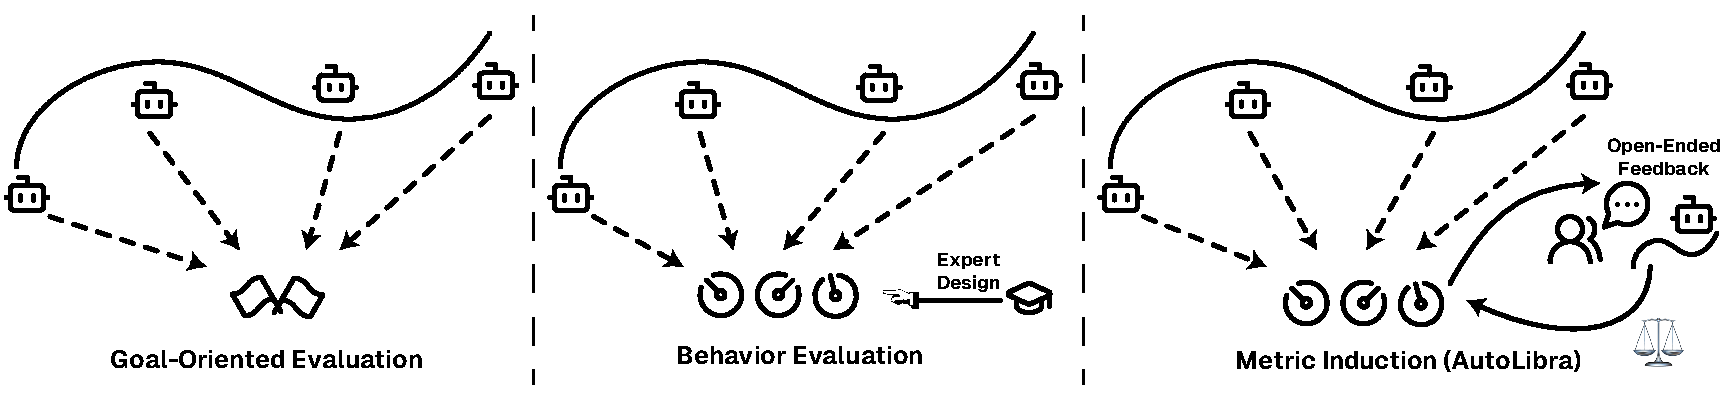
\includegraphics[width=0.5\textwidth]{figs/autolibra.pdf}
   \caption{Comparison of AutoLibra with existing agent evaluation paradigms.}
\end{wrapfigure}


Feedback is critical for human self-assessment and improvement \citep{nicol2006formative}.

Compared to the scarce reward
we get from achieving goals, these metrics offer a lens for self-reflection on the
strengths and weaknesses of ourselves and a ladder for self-improvement.
In this paper, we ask:
\textbf{can we automatically induce metrics to evaluate and improve language agents from natural language feedback?} 

   
The current evaluation of large language model (LLM) agents and reward modeling often fall
into two paradigms: (1) goal-oriented evaluation --
\emph{whether the agents have fulfilled the given task},
\emph{e.g.} \citet{zhouwebarena,jimenezswe,chan2024mle,paglieri2024balrog}
and (2) behavior evaluation -- \emph{how well the agents do on heuristically designed dimensions},
\emph{e.g.} \citet{zhousotopia,shao2024collaborative,pan2025why}. 
Goal-oriented evaluation is often verifiable, but it is not fine-grained or comprehensive enough
to diagnose agents' behavior problems or find the bottlenecks for improvements. 
While behavior evaluation complements it, it requires manual design of the metrics by experts,
which is time-consuming, may not align with users' opinions, and often not concrete enough. 

We introduce AutoLibra \protect\includegraphics[height=1em]{figs/scale.png}, an automatic metric induction method,
as a new paradigm for agent evaluation and improvement.
This method offers behavior evaluation for agents, while (1) automating the metric creation process with LLMs, 
(2) optimizing the alignment through searching for a set of metrics to cover human feedback with minimal redundancy,
and (3) providing concrete examples of good and bad behaviors for each metric to improve the
LLM-as-a-Judge's performance. 

AutoLibra takes in agent trajectories along with human open-ended feedback, and generates a set of metrics, each with a name, description, and a list of good behavior examples, and bad behavior examples. AutoLibra 



\begin{wrapfigure}{r}{0.7\textwidth}
    \centering
    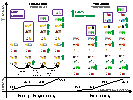
\includegraphics[width=0.7\textwidth]{figs/autolibra-teaser.pdf}
    \caption{Caption}
    \label{fig:enter-label}
\end{wrapfigure}


\section{AutoLibra\protect\includegraphics[height=1em]{figs/scale.png}}

\begin{figure}[!t]
    \centering
    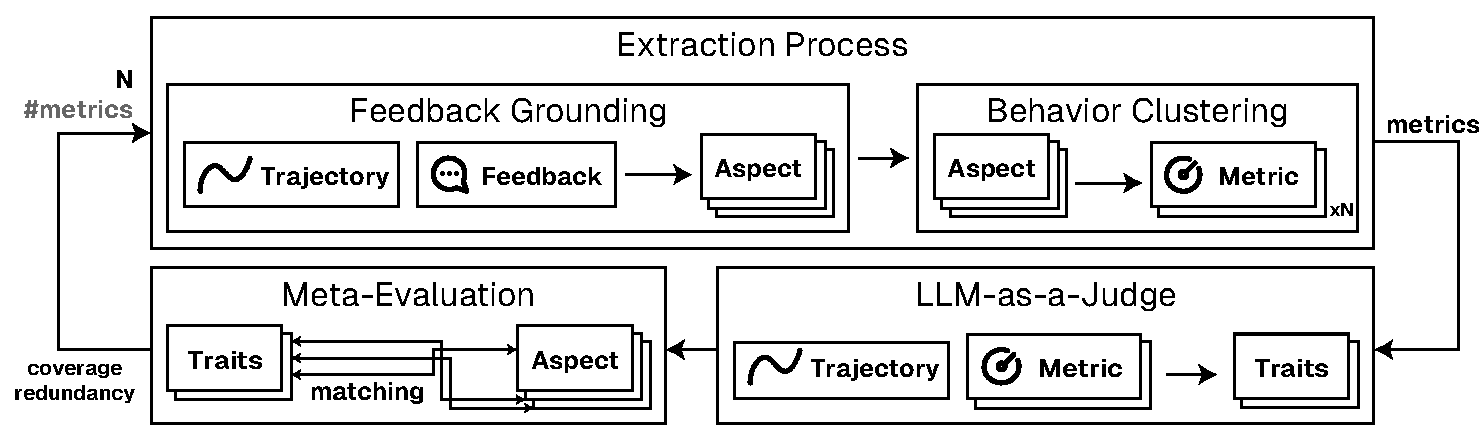
\includegraphics[width=\textwidth]{figs/autolibra-pipeline.pdf}
    \caption{AutoLibra pipeline. AutoLibra consists of three major components: Extraction Process
    turns annotated agent trajectories into metrics, LLM-as-a-Judge evaluates the agent trajectories
    based on the induced metrics, and Meta-Evaluation Process measures the quality of induced metrics
    through matching the detect agent traits with grounded feedback aspects.
    }
    \label{fig:autolibra-pipeline}
\end{figure}

To address the limitations of existing evaluation paradigms, we seek to design an evaluation method that 
meets the following desiderata: (1) \emph{data-driven}: this makes sure that the metrics are grounded
in the real agent behavior and human opinions, (2) \emph{generic}: applicable to various agent domains 
without the need for domain-specific design, (3) \emph{self-verifiable}: this provides guarantee that the 
induced metrics can be used in LLM-as-a-Judge to generate human-aligned evaluation. 

As illustrated in Fig. \ref{fig:autolibra-pipeline}, AutoLibra achieves these desiderata through a closed-loop pipeline
consisting of three major steps: \textbf{Extraction Process} first grounds the human feedback
for each trajectory into aspects (\S\ref{sec:grounding}), and then clusters the aspects into $N$ metrics(\S\ref{sec:clustering}).
\textbf{LLM-as-a-Judge} gives each trajectory scores for the induced metrics, the combinations of
metrics and scores becoming the traits of the agents (\S\ref{sec:llm-judge}).
Finally, \textbf{Meta-Evaluation Process} measures the quality of induced metrics through matching
the detected agent traits with aspects in the human feedback (\S\ref{sec:meta-evaluation}).
To optimize for the lowest redundancy with highest coverage, we control the number of metrics 
through a hyperparameter $N$ in the clustering step (\S\ref{sec:metric-optimization}). AutoLibra also supports
an interative metric induction process, where as the agent is optimized, new metrics can be addeding 
to the existing metrics (\S\ref{sec:iterative-induction}).

\subsection{Feedback grounding}
\label{sec:grounding}
The feedback of human annotators could contains multiple aspects, e.g. \textsf{AI agent was pretty good
on giving me a consistent itinerary and vacation plan, although It froze on the last couple of minutes.},
collected from human annotators in CoGym \citep{shao2024collaborative}, contains a positive aspect
about the agent's ability to generate a consistent itinerary, and a negative aspect about the agent freezing
at the end. Here we define an \emph{aspect} as a triple $(\texttt{behavior}, \texttt{feedback}, \texttt{sign})$.
In the positive aspect of the previous example, the \texttt{behavior} is the agent's actions to create
a 20-day itinerary for Maldives, the \texttt{feedback} is that the itinerary created is consistent, 
and the \texttt{sign} is positive. 



\subsection{Behavior clustering}
\label{sec:clustering}

\subsection{LLM-as-a-Judge}
\label{sec:llm-judge}

\subsection{Meta-evaluation}
\label{sec:meta-evaluation}

\subsection{Metric optimization}
\label{sec:metric-optimization}

\subsection{Iterative metric induction}
\label{sec:iterative-induction}

\section{The Lens \protect\includegraphics[height=1em]{figs/microscope.png}: Agent evaluation with AutoLibra}
\label{sec:lens}

In this section, we use AutoLibra as a lens to provide grounded, behavior-salient insights into agent trajectories. We evaluate coverage of induced metrics have and they can be generalized to novel human feedback.

Intuitively, coverage and redundancy grow as the number of metrics increases. However, we observe diminishing coverage gains past $N=6$ to $N=10$, while redundancy continues to increase.
On held-out human feedback (mentioned in \S\ref{sec:collecting-human-feedback}), coverage and redundancy are marginally worse than the from feedback used to induce the metrics, which demonstrates that AutoLibra produces metrics that are generalizable to arbitrary agent trajectories. We also find \diyi{do you have ablation results here in a detailed fashion, instead of briefly saying it changes from 5 to 30\%?} that LLM-as-a-Judge is improved by use of the good- and bad-behavior examples in the metrics -- across all datasets, not using the examples reduces the coverage significantly (5\% to 30\%). 

\diyi{i recommend creating a table to lay out the original metrics from each work, and the new metrics you induced, to give readers a clear read.}


\citet{shao2024collaborative} organize the failure modes in CoGym into five main categories. We find that the metrics induced on CoGym from the user feedback with AutoLibra cover similar categories, demonstrating the consistenty of AutoLibra as a metric extraction tool: \textit{Communication clarity and user interaction} belongs to Communication,  \textit{Adherence to instructions and consistency} belongs to Situational Awareness, \textit{Adaptability and responsiveness to feedback} belongs to Planning, \textit{Search accuracy and content relevance} belongs to Environment Awareness, and \textit{User preference query and incorporation} belongs to Personalization. All five metrics are more concrete and fine-grained than the larger categories in CoGym; we also discover the following metrics that are not mentioned in the break-down analysis in the CoGym paper:
\textit{Response time and efficiency}, \textit{Itinerary and report detail quality}, and \textit{Formatting and presentation consistency}. We note that this comparison shows the complementary characteristics of automatically 
induced metrics, which are more concrete on the issues that users are noticing, while the expert-designed categories measure the high-level capabilities of AI agents. 

Similarly, \citet{zhousotopia} propose seven dimensions for evaluating social intelligence in AI agents. Among the induced metrics, 3 metrics map well to behaviors in Sotopia-Eval: \textit{Conversational Naturalness and Efficiency}, \textit{Personality Consistency and Alignment}, \textit{Contextual Integration of Identity and Personal Background}, while metrics like \textit{Negotiation Tactics and Strategic Adaptability} and \textit{Responsiveness and Conversational Termination} are not captured in any of the dimensions of Sotopia-Eval. 

For web navigation tasks, AutoLibra also discovers metrics including \textit{Access Barrier Handling}, \textit{Error Recovery and Iterative Adjustment}, \textit{Step Efficiency and Action Redundancy} which much more closely reflect emergent agent behavior than the failure analysis categories proposed in previous work \citep{he2024webvoyager,zhou2024proposeragentevaluatorpaeautonomousskilldiscovery}, where they are often classified as ``navigation stuck''. %Understanding the cause of the navigation failure is access barrier such as CAPTCHA or error recovery is important for improving the agents. 

%\diyi{i thought we also had some insights on how these metrics can be generalized across similar tasks. Is this highlighted somewhere? Phil: in theory handled in section 4}



\section{The Ladder \protect\includegraphics[height=1em]{figs/ladder.png}: Agent improvement with AutoLibra}
\label{sec:ladder}

In this section, we use AutoLibra to iteratively improve agent performance (as a 'ladder') through prompt engineering and fine-tuning, to comprehensively study whether the induced metrics are good optimization targets. 
%On a text-game task (Baba-Is-AI), \diyi{delete this sentence of results and use the following subsections to share about your results, to avoid repetition. } we find that optimizing prompts driven by iteratively induced metrics improves the performance of state-of-the-art agents significantly. Similarly, on web navigation tasks, we find that fine-tuning on the data selected by the induced metrics can iteratively improve the agent performance better than goal-oriented scores. 
Fig. \ref{fig:autolibra-training} illustrates the results. In all experiments, GPT-4o is used as (at the time of writing) it has a leading bench on the BALROG benchmark \cite{paglieri2024balrog}; Claude-3.5-Sonnet is used in ablations as it has a comparable bench (32.3 \% vs. 32.6 \%), respectively.

\subsection{Agent prompt engineering case study: Baba-Is-AI}
\label{sec:Baba-Is-AI}

Baba-Is-AI \citep{cloos2024babaaibreakrules} is a grid world game which is especially challenging for LLM agents since it requires navigation and interaction with blocks that modify in-environment rules. Implementation-specific details are discussed in more detail in Appendix \ref{appendix:baba_is_ai_rules}.


% \begin{figure}[ht]
%     \centering
%     \includegraphics[scale=0.5]{figs/babaisai_env.png}
%     \caption{Example of the Baba-Is-AI environment. In this task (two\_room-break\_stop-make\_win-distr\_obj-irrelevant\_rule), the agent has to break the "wall is stop" rule and push the "key" rule block next to "is win" to assemble the win rule, then touch the key to win. Pushing the "door" rule block would be a mistake, as no door object is present.}
%     \label{fig:babaisai_env}
% \end{figure}

% \subsection{AutoLibra for Baba-Is-AI improvement}


In performing iterative agent improvement with AutoLibra, a full cycle of the AutoLibra ladder pipeline is considered one \textit{Iteration}, for which the pseudocode and environment configuration are detailed in Appendix \ref{appendix:algo1}.

\begin{wraptable}[19]{r}{0.60\textwidth} % 'r' for right, adjust the width as needed
\centering
\small
\vspace{-30pt}
\begin{tabular}{ccl}
\toprule
\multicolumn{1}{c}{Emoji}& 
\multicolumn{1}{c}{It.} & 
\multicolumn{1}{l}{Metric} \\
\midrule
\rowcolor{gray!10} \includegraphics[scale=0.07]{figs/emojis/emoji_1.png} & 0 & Win Condition Recognition \\
\midrule
\rowcolor{gray!10} \includegraphics[scale=0.07]{figs/emojis/emoji_2.png} & 0 & Rule Modification \\
\midrule
\rowcolor{gray!10} \includegraphics[scale=0.07]{figs/emojis/emoji_3.png} & 0 & Direct Navigation Efficiency \\
\midrule
\rowcolor{gray!10} \includegraphics[scale=0.07]{figs/emojis/emoji_4.png} & 0 & Context-Sensitive Decision Making \\
\midrule
\rowcolor{gray!30} \includegraphics[scale=0.07]{figs/emojis/emoji_5.png} & 1 & Win Rule Construction \\
\midrule
\rowcolor{gray!30} \includegraphics[scale=0.07]{figs/emojis/emoji_6.png} & 1 & Selective Interaction With Relevant Objects  \\
\midrule
\rowcolor{gray!30} \includegraphics[scale=0.07]{figs/emojis/emoji_7.png} & 1 & Rule Manipulation and Execution  \\
\midrule
\rowcolor{gray!60} \includegraphics[scale=0.07]{figs/emojis/emoji_8.png} & 2 & Subtask Coordination \\
\midrule
\rowcolor{gray!90} \includegraphics[scale=0.07]{figs/emojis/emoji_9.png} & 3 & Immovable Interaction \\
\bottomrule
\end{tabular}
\caption{Metrics and Turn of Induction \newline for Baba-Is-AI}
\label{tab:metrics}
\end{wraptable}

% \begin{figure}[ht]
%     \centering
%     \begin{minipage} % First table in a minipage taking 45% of the text width
%         \begin{wraptable}[19]{r}{0.60\textwidth} % 'r' for right, adjust the width as needed
\centering
\small
\vspace{-30pt}
\begin{tabular}{ccl}
\toprule
\multicolumn{1}{c}{Emoji}& 
\multicolumn{1}{c}{It.} & 
\multicolumn{1}{l}{Metric} \\
\midrule
\rowcolor{gray!10} \includegraphics[scale=0.07]{figs/emojis/emoji_1.png} & 0 & Win Condition Recognition \\
\midrule
\rowcolor{gray!10} \includegraphics[scale=0.07]{figs/emojis/emoji_2.png} & 0 & Rule Modification \\
\midrule
\rowcolor{gray!10} \includegraphics[scale=0.07]{figs/emojis/emoji_3.png} & 0 & Direct Navigation Efficiency \\
\midrule
\rowcolor{gray!10} \includegraphics[scale=0.07]{figs/emojis/emoji_4.png} & 0 & Context-Sensitive Decision Making \\
\midrule
\rowcolor{gray!30} \includegraphics[scale=0.07]{figs/emojis/emoji_5.png} & 1 & Win Rule Construction \\
\midrule
\rowcolor{gray!30} \includegraphics[scale=0.07]{figs/emojis/emoji_6.png} & 1 & Selective Interaction With Relevant Objects  \\
\midrule
\rowcolor{gray!30} \includegraphics[scale=0.07]{figs/emojis/emoji_7.png} & 1 & Rule Manipulation and Execution  \\
\midrule
\rowcolor{gray!60} \includegraphics[scale=0.07]{figs/emojis/emoji_8.png} & 2 & Subtask Coordination \\
\midrule
\rowcolor{gray!90} \includegraphics[scale=0.07]{figs/emojis/emoji_9.png} & 3 & Immovable Interaction \\
\bottomrule
\end{tabular}
\caption{Metrics and Turn of Induction \newline for Baba-Is-AI}
\label{tab:metrics}
\end{wraptable} % Your first table
%     \end{minipage}%
%     \hfill % Adds some horizontal space between the tables
%     \begin{minipage} % Second table in a minipage taking 45% of the text width
%         \centering
%         \renewcommand{\arraystretch}{1.5} 
\begin{table}[h!]

\centering
\begin{tabular}{|>{\raggedright\arraybackslash}p{6cm}|c|c|c|c|}
\hline
\textbf{Turn} & \textbf{0} & \textbf{1} & \textbf{2} & \textbf{3} \\
\hline
\textbf{Babaisai Score GPT-4o} & 0.30 & 0.40 & 0.43 & 0.55 \\
\hline
\textbf{Babaisai Score Claude 3.5 Sonnet} & 0.35 & 0.40 & 0.45 & 0.55 \\
\hline
\textbf{Average Env. Steps} & 79 & 63 & 60 & 51 \\
\hline
\end{tabular}
\caption{Babaisai Scores and Average Environment Steps}
\label{tab:heldout}
\end{table} % Your second table
%     \end{minipage}
%     \caption{Tables side by side}
% \end{figure}

\paragraph{Results}

Held-out task performance increased by 25\% to 55\% between \textit{Iteration 0} and \textit{Iteration 3}, with each iteration resulting in greater performance than the last (Full held-out task results tabulated in Appendix \ref{appendix:heldout}); \textbf{this result was replicated across several tested models}. This represents a substantial increase compared to the highest base model performance of 33\% on Baba-Is-AI \citep{paglieri2024balrog}, demonstrating that improvements realized by AutoLibra are generalizable to unseen tasks and validating the utility of the framework in augmenting the performance of agents in highly diverse environments. Among induced metrics (Table \ref{tab:metrics}), agent performance increases correspondingly to code changes targeting those metrics, an example being \texttt{Win Condition Recognition} \includegraphics[scale=0.07]{figs/emojis/emoji_1.png}, which increases from 28\% to 50\% from \textit{Iterations 0-1} after few-shot prompting is introduced to demonstrate identifying a win condition rule, with a full list of improvements and examples presented in Appendix \ref{appendix:baba_is_ai_obs}. The high correlation between induced metrics, targeted changes to agent code, and improvements in the agent performance on those metrics validates the fine-grainedness and human-interpretability of AutoLibra metrics, and demonstrates its utility in targeted improvement of agent behaviors.

Similarly to results observed in Section 3, induced metrics are observed to capture the behavior of the agent increasingly well with additional iterations, with coverage increasing from 65\% at \textit{Iteration 0} to 92\% at \textit{Iteration}, while mean redundancy remains 56\% across all iterations. The trajectory performance also improved significantly, with the average number of steps per task (capped at 100) decreasing from 79 to 51, indicating that the agent's reasoning performance and efficiency improved as a result of the code changes made in each iteration.

Qualitative observation of agent trajectories reveals behaviors commensurate with induced metric scores; the agent random-walks in \textit{Iteration 0}, navigates towards specific objectives but gets stuck or trapped in a loop on long-horizon tasks in \textit{Iteration 1} and \textit{Iteration 2}, and fully understands basic subtasks (atomic goals on the critical path to environment completion) and the correct order of subtasks to successfully complete an environment in \textit{Iteration 3}.

A per-metric score breakdown is listed in Appendix \ref{appendix:babaisai}, and a full per-iteration documentation of code changes and results is presented in Appendix \ref{appendix:baba_is_ai_obs}.

% \subsubsection{Held-Out Task Performance}

\paragraph{Ablation Study}

To evaluate the generalization of the improvements realized by AutoLibra, we conducted an ablation study where the performance of the agent improved by AutoLibra was evaluated on unseen Baba Is You levels, arbitrary LLMs, and entirely new environments.

\textbf{Model Generalization} When replacing GPT-4o with Claude-3-5 as the LLM used in the agent (Appendix \ref{appendix:heldout}), performance was found to be similar across all iterations, with held-out task performance increasing by 20\% to 55\% between \textit{Iteration 0} and \textit{Iteration 3} and qualitatively similar trajectory performance and agent behaviors observed between the two LLMs. This demonstrates that the improvements realized by AutoLibra are generalizable to other LLMs, and that the induced metrics are robust to changes in the underlying LLM. %\diyi{this result is important - i suggest putting it back to support how the metrics generalize across different LLMs.}

\textbf{Environment Generalization} AutoLibra-Ladder was further evaluated in MiniHack, an environment whose tasks and action space are more complex than Baba-Is-AI \citep{samvelyan2021minihackplanetsandboxopenended}. Across three iterations, the task completion rate was observed to increase to 25\%, an improvement of 15\% versus the baseline of 10\%,  validating AutoLibra's general utility in improving agent performance; full results are available in Appendices \ref{appendix:minihack_rules}-\ref{appendix:minihack_obs}.
%\diyi{use a paragraph title to illustrate that this is about generalization? i also didn't quite follow why minihack is only summarized using these two sentences. if you want to emphasize it, explain it clearly; otherwise, no need to mention it? } 


\subsection{Agent finetuning case study: web navigation}
%\diyi{i found the model choices quite arbitrary -- first, it wasn't clear to me what models are used in 4.1, some of which seems to be gpt-4o etc; in s4.2, we used llama-8b, so my question is: what's the rationale behind these model selections? we can't just ask readers to go to appendix for these super critical choices.}
We choose web navigation as the domain of the fine-tuning application to leverage the diverse trajectory dataset NNetNav-live \citep{Murty2025NNetNav} to use our induced metrics as the data selection method. Using Llama-8b-nnetnav-live \footnote{Llama-8b-nnetnav-live is selected due to being the highest-scoring model on WebVoyager} as the baseline model in each iteration, we sample 40 trajectories from the current agent policy executing 40 random tasks in NNetNav-live to give feedback and iteratively induce new metrics. After the new metrics are induced, we sample one trajectory for each task in NNetNav-live, and select the ones with top 10\% sum scores of all metrics for finetuning the agent policy. Note that the tasks in NNetav-live are discovered through an exploration algorithm, with no overlap with WebVoyager dataset \citep{he2024webvoyager}. We test the agents' performance on WebVoyager dataset; success rates are shown in Fig. \ref{fig:autolibra-training}. As a baseline, we also finetune the agent policy on trajectories selected with top 10\% goal-oriented scores using the evaluation method introduced in \citep{pan2024autonomous}. However, we do not observe significant improvement on top of Llama-8b-nnetnav-live. This shows that the metrics iteratively induced by AutoLibra also serve as better optimization target than goal-oriented evaluation scores. The metrics induced in each iteration are in Appendix Table \ref{tab:app_nnetnav_metrics}.
\section{Related Work}
AutoLibra unifies three areas of research: it draws inspiration from \textit{thematic analysis} to create \textit{nautral language-derived evaluation metrics} to evaluate \textit{AI agents}. 

\paragraph{Evaluating AI agents} Much of the work in AI agent evaluation builds a benchmark which contains both task suites and evaluation metrics. In addition to the data sets we used in this paper, SWE-Bench \citep{jimenezswe} uses human-written unit tests as evaluation metrics; Embodied Agent Interface \citep{li2024embodied} provides fine-grained evaluation for LLM-based embodied agents; $\tau$-Bench \citep{yao2024tau} compares database states for evaluation. In contrast to these, AutoLibra is a task-agnostic method for generating metrics. 

\paragraph{Learning from natural language feedback} Recently, there is substantial interest in training agents from natural language feedback. \citet{chen2024learning} propose an imitation learning method for learning from human feedback; Text2Reward \citep{xietext2reward} uses code generation to generate robot reward functions from open-ended human feedback; \citet{shi2024yell} propose a new model architecture to incorporate human feedback into policy learning. Unlike these papers, AutoLibra induces metrics from all annotated instances and generates metrics that are useful for both evaluation and agent fine-tuning.
\paragraph{Automatic thematic analysis} Thematic analysis is a powerful tool for qualitative study through coding and iterative creating themes. \citet{gauthier2022computational} provide computational tools to aid this process; \citet{hong2022scholastic} and \citet{gebreegziabher2023patat} explore human-AI collaboration in thematic analysis; LLooM \citep{lam2024concept}, is an automatic method for concept induction, is closest to and influences our approach. This paper completes the loop of concept induction by using the meta-evaluation step to optimize the induced metrics, and apply this social science technique to agent evaluation. 
\documentclass[../main.tex]{subfiles}

\begin{document}

\section{Conclusion and Future Work}
This work introduces AutoLibra, a new paradigm for agent evaluation, one of
the first works to explore adaptable trajectory-derived evaluation heuristics,
offering substantial advantages in agent training over traditional end-to-end
evaluation. We find that this framework is generalizable to a diverse range of agent
tasks, provides new insights into agent behaviors, and identifies strong optimization
targets for agent improvement. There are a few directions for further extending
and applying this framework.
(1) \textbf{Behavior-centric evaluation} AutoLibra leads a \emph{paradigm shift}
from end-to-end agent evaluation (analogous to ``integration tests'' in software
development) to evaluation with granular metrics that measure agents' concrete behaviors
(analogous to ``unit tests''). Future work can study whether this process can be
improved through better human-AI collaboration.
(2) \textbf{Sub-trajectory feedback from humans} In AutoLibra, we label each
trajectory with one piece of feedback, and ground it into the agents' concrete
behavior which is at the sub-trajectory level. In the future, researchers can
let users directly give feedback for one or multiple steps in the trajectory, which
should lead to better feedback grounding results. Similarly, user feedback can be
collected during the interaction instead of after the agent has completed the tasks,
which is a more user-friendly way to gather high quality feedback data.
(3) \textbf{Wider exploration of agent improvement methods} In this paper, we only
explored non-parametric for agent improvement to show the utility of AutoLibra. Future work can use AutoLibra to provide dense rewards for individual
steps, and use reinforcement learning to train agents with these dense rewards.

\end{document}


\section*{Limitation and Ethics Statement}
The scope of this paper is text-based agents, which does not include agents with multimodal observation or action spaces. Within human-aided experiments, we are also limited by the diversity of human annotators. The annotation of the data in this paper, except for the feedback collected by \citet{shao2024collaborative}, is done by the authors, who are experts in AI agents. We do not address the effect of the experience of the annotators on the induced metrics. Finally, induced metrics should be used with caution, these could reflect the internal biases of the LLMs used to extract them. 



\bibliography{colm2025_conference}
\bibliographystyle{colm2025_conference}

\appendix
\section{Appendix}
\appendix

\appendix
\section*{Content of Appendix}
\begin{itemize}
    \item[\ref{appendix:babaisai}] Baba-is-ai Metric Scores
    \item[\ref{appendix:minihack}] Minihack Metric Scores
\end{itemize}

\section{Baba-is-ai Metric Performance}
\label{appendix:babaisai}
% Function to generate color based on percentage value
\newcommand{\cellcolorpercent}[1]{%
  \ifdim #1 pt < 10 pt \cellcolor{red!90}%
  \else\ifdim #1 pt < 20 pt \cellcolor{red!80}%
  \else\ifdim #1 pt < 30 pt \cellcolor{red!70}%
  \else\ifdim #1 pt < 40 pt \cellcolor{red!60}%
  \else\ifdim #1 pt < 50 pt \cellcolor{red!50}%
  \else\ifdim #1 pt < 60 pt \cellcolor{yellow!40}%
  \else\ifdim #1 pt < 70 pt \cellcolor{yellow!30}%
  \else\ifdim #1 pt < 80 pt \cellcolor{green!30}%
  \else\ifdim #1 pt < 90 pt \cellcolor{green!50}%
  \else\ifdim #1 pt < 100 pt \cellcolor{green!70}%
  \else\cellcolor{green!90}%
  \fi\fi\fi\fi\fi\fi\fi\fi\fi\fi
}

\makeatletter
\newcommand{\thickhline}{%
    \noalign {\ifnum 0=`}\fi \hrule height 3pt
    \futurelet \reserved@a \@xhline
}
\newcolumntype{"}{@{\hskip\tabcolsep\vrule width 1pt\hskip\tabcolsep}}
\makeatother

\renewcommand{\arraystretch}{1.5} 
\begin{table}[ht]
\centering
\begin{tabular}{|>{\arraybackslash}p{5cm}|>{\arraybackslash}p{1.5cm}|c|c|c|c|}
\hline
\rowcolor[HTML]{C0C0C0} 
\textbf{} & \textbf{Iteration} & \textbf{0} & \textbf{1} & \textbf{2} & \textbf{3} \\ \hline
Win Condition Recognition & \includegraphics[scale=0.07]{figs/emojis/emoji_1.png} & \cellcolorpercent{27.78} \textbf{27.78\%} & \cellcolorpercent{50.00} \textbf{50.00\%} & \cellcolorpercent{88.89} \textbf{88.89\%} & \cellcolorpercent{94.44} \textbf{94.44\%} \\ \hline
Rule Modification & \includegraphics[scale=0.07]{figs/emojis/emoji_2.png} & \cellcolorpercent{5.56} \textbf{5.56\%} & \cellcolorpercent{11.11} \textbf{11.11\%} & \cellcolorpercent{27.78} \textbf{27.78\%} & \cellcolorpercent{44.44} \textbf{44.44\%} \\ \hline
Direct Navigation Efficiency & \includegraphics[scale=0.07]{figs/emojis/emoji_3.png} & \cellcolorpercent{5.56} \textbf{5.56\%} & \cellcolorpercent{12.50} \textbf{12.50\%} & \cellcolorpercent{12.50} \textbf{12.50\%} & \cellcolorpercent{44.44} \textbf{44.44\%} \\ \hline
Context-Sensitive Decision Making & \includegraphics[scale=0.07]{figs/emojis/emoji_4.png} & \cellcolorpercent{11.11} \textbf{11.11\%} & \cellcolorpercent{12.50} \textbf{12.50\%} & \cellcolorpercent{12.50} \textbf{12.50\%} & \cellcolorpercent{38.89} \textbf{38.89\%} \\ \hline
Win Rule Construction & \includegraphics[scale=0.07]{figs/emojis/emoji_5.png} & - & \cellcolorpercent{0.00} \textbf{0.00\%} & \cellcolorpercent{0.00} \textbf{0.00\%} & \cellcolorpercent{5.56} \textbf{5.56\%} \\ \hline
Selective Interaction With Relevant Objects & \includegraphics[scale=0.07]{figs/emojis/emoji_6.png} & - & \cellcolorpercent{27.78} \textbf{27.78\%} & \cellcolorpercent{44.44} \textbf{44.44\%} & \cellcolorpercent{88.89} \textbf{88.89\%} \\ \hline
Rule Manipulation and Execution & \includegraphics[scale=0.07]{figs/emojis/emoji_7.png} & - & \cellcolorpercent{5.56} \textbf{5.56\%} & \cellcolorpercent{27.78} \textbf{27.78\%} & \cellcolorpercent{33.33} \textbf{33.33\%} \\ \hline
Subtask Coordination & \includegraphics[scale=0.07]{figs/emojis/emoji_8.png} & - & - & \cellcolorpercent{11.11} \textbf{11.11\%} & \cellcolorpercent{33.33} \textbf{33.33\%} \\ \hline
Immovable Interaction & \includegraphics[scale=0.07]{figs/emojis/emoji_9.png} & - & - & - & \cellcolorpercent{66.67} \textbf{66.67\%} \\ 
\thickhline 
\multicolumn{2}{|c|}{Coverage} & 65\% & 83\% & 85\% & 92\% \\ \hline
\multicolumn{2}{|c|}{Redundancy} & 58\% & 59\% & 47\% & 59\% \\ \hline
\end{tabular}
\caption{Metric Performance for baba-is-ai AutoLibra Iterations 0-3}
\label{tab:metric_perf}
\end{table}


\section{Minihack Metric Performance}
\label{appendix:minihack}
\renewcommand{\arraystretch}{1.5}
\begin{table}[ht]
	\centering
	\begin{tabular}{|>{\arraybackslash}p{6cm}|>{\arraybackslash}p{1.5cm}|c|c|c|}
		\hline
		\rowcolor[HTML]{C0C0C0} \textbf{}                & \textbf{Iteration}                                   & \textbf{0}                                & \textbf{1}                                & \textbf{2}                                \\
		\hline
		% Row 1
		Target Navigation Effectiveness                  & \includegraphics[scale=0.09]{figs/emojis/mini_1.png} & \cellcolorpercent{16.67} \textbf{16.67\%} & \cellcolorpercent{8.33} \textbf{8.33\%}   & \cellcolorpercent{41.67} \textbf{41.67\%} \\
		\hline
		% Row 2
		Efficient Exploration and Map Memory Utilization & \includegraphics[scale=0.07]{figs/emojis/mini_2.png} & \cellcolorpercent{16.67} \textbf{16.67\%} & \cellcolorpercent{0.00} \textbf{0.00\%}   & \cellcolorpercent{25.00} \textbf{25.00\%} \\
		\hline
		% Row 3
		Hazard Awareness and Equipment Utilization       & \includegraphics[scale=0.09]{figs/emojis/mini_3.png} & \cellcolorpercent{0.00} \textbf{0.00\%}   & \cellcolorpercent{0.00} \textbf{0.00\%}   & \cellcolorpercent{0.00} \textbf{0.00\%}   \\
		\hline
		% Row 4
		Boulder Manipulation Strategy                    & \includegraphics[scale=0.09]{figs/emojis/mini_4.png} & \cellcolorpercent{0.00} \textbf{0.00\%}   & \cellcolorpercent{0.00} \textbf{0.00\%}   & \cellcolorpercent{0.00} \textbf{0.00\%}   \\
		\hline
		% Row 5
		Combat Engagement and Survival                   & \includegraphics[scale=0.09]{figs/emojis/mini_5.png} & \cellcolorpercent{8.33} \textbf{8.33\%}   & \cellcolorpercent{8.33} \textbf{8.33\%}   & \cellcolorpercent{25.00} \textbf{25.00\%} \\
		\hline
		% Row 6
		Role-Specific Ability Utilization                & \includegraphics[scale=0.07]{figs/emojis/mini_6.png} & \cellcolorpercent{0.00} \textbf{0.00\%}   & \cellcolorpercent{0.00} \textbf{0.00\%}   & \cellcolorpercent{0.00} \textbf{0.00\%}   \\
		\hline
		% Row 7
		Spatial Awareness and Interpretation             & \includegraphics[scale=0.08]{figs/emojis/mini_7.png} & {-}                                       & \cellcolorpercent{16.67} \textbf{16.67\%} & \cellcolorpercent{58.33} \textbf{58.33\%} \\
		\hline
		% Row 8
		Object Pickup Efficiency                         & \includegraphics[scale=0.08]{figs/emojis/mini_8.png} & {-}                                       & \cellcolorpercent{0.00} \textbf{0.00\%}   & \cellcolorpercent{0.00} \textbf{0.00\%}   \\
		\hline
		% Row 9
		Giant Rats Encounter Handling                    & \includegraphics[scale=0.08]{figs/emojis/mini_9.png} & {-}                                       & {-}                                       & \cellcolorpercent{25.00} \textbf{25.00\%} \\
		\thickhline                                       % Coverage and Redundancy
		\multicolumn{2}{|c|}{Coverage}                   & 82.89\%                                              & 81.82\%                                   & 87.84\%                                    \\
		\hline
		\multicolumn{2}{|c|}{Redundancy}                 & 61.11\%                                              & 65.63\%                                   & 71.30\%                                    \\
		\hline
	\end{tabular}
	\caption{Metric Performance for MiniHack AutoLibra Iterations 0–2}
	\label{tab:metric_mini_perf}
\end{table}

\end{document}
